\section{\SecAdvanceMapprojectionSetting} \label{subsec:adv_mapproj}
%------------------------------------------------------
\scalerm では、まず実距離に基づいた格子点が配置され、その格子点位置と緯度経度基準点の情報を元に、
それぞれの投影法を用いた際の各格子点での緯度・経度座標が計算される。
緯度・経度情報は、すべてのSCALEのNetCDF形式の出力ファイルに含まれている。\\
計算領域の位置と投影法は、設定ファイルの\nmitem{PARAM_MAPPROJ}の項目を編集することで設定できる。
\textcolor{red}{\bf この設定も、pp\_***.conf、init\_***.conf、run\_***.confの設定ファイルの間で
必ず一致させなければならない。}はじめに下記の例をもとに説明する。\\

\noindent {\small {\gt
\ovalbox{
\begin{tabularx}{140mm}{l}
\verb|&PARAM_MAPPROJ| \\
\verb| MPRJ_basepoint_lon = 138.727778D0,| \\
\verb| MPRJ_basepoint_lat = 35.360556D0,| \\
\verb| MPRJ_type          = 'MER',| \\
\verb|/| \\
\end{tabularx}
}}}\\

\begin{table}[b]
\begin{center}
\caption{SCALEで選択できる地図投影法}
\begin{tabularx}{150mm}{|l|X|} \hline
 \rowcolor[gray]{0.9} \verb|MPRJ_type| & 地図投影法 \\ \hline
 \verb|NONE| & 地図投影なし(理想実験用)、デフォルト \\ \hline
 \verb|LC|   & ランベルト正角円錐図法              \\ \hline
 \verb|PS|   & ポーラーステレオ図法                \\ \hline
 \verb|MER|  & メルカトル図法                     \\ \hline
 \verb|EC|   & 正距円筒図法                       \\ \hline
\end{tabularx}
\label{tab:map_proj}
\end{center}
\end{table}

\noindent
まず\nmitem{MPRJ_basepoint_lat}と\nmitem{MPRJ_basepoint_lon}は、
計算領域の中心の緯度・経度を表す。
SCALE-RMでは、北緯を正、南緯を負の値として表現し、
経度は0度を起点に右回りで表現するため、
この設定例では計算領域の
中心が北緯35.360556度、東経138.727778度に位置することになる。
この場所を中心に指定された大きさで、計算領域が設定される。\\
\nmitem{MPRJ_type}は、地図投影法の種類を表しており、\verb|MER|はメルカトル図法を意味する。
\scalerm で現在選択できる地図投影法とその指定文字列は表\ref{tab:map_proj}のとおりである。
メルカトル図法を用いた場合、投射する円筒に接する基準緯線は\nmitem{MPRJ_M_lat}で任意の値に設定する。
通常、基準緯線は赤道にとることが多いが、基準緯線に近いほど歪みが少なく正確に記述できるので、
\nmitem{MPRJ_M_lat}を指定しない場合は\nmitem{MPRJ_basepoint_lat}が基準緯線として用いられる。

投影法の中でも利用頻度が高いランベルト正角円錐図法の設定について以下に説明する。
ここでは、現実大気実験チュートリアルで使用した\verb|run.conf|ファイルを例に挙げる。\\

{\small {\gt
\ovalbox{
\begin{tabularx}{140mm}{l}
\verb|&PARAM_MAPPROJ| \\
\verb| MPRJ_basepoint_lon = 135.220404D0,| \\
\verb| MPRJ_basepoint_lat = 34.653396D0,| \\
\verb| MPRJ_type          = 'LC',| \\
\verb| MPRJ_LC_lat1       =  30.00D0,| \\
\verb| MPRJ_LC_lat2       =  40.00D0,| \\
\verb|/| \\
\end{tabularx}
}}}\\

\noindent
\scalerm では、2標準緯線型の投影方法を採用している。
両標準緯線に挟まれた領域では、
緯線・経線の長さの比が地球楕円体面上における長さの比と近くなるように調節される。
南側、北側の標準緯線はそれぞれ\nmitem{MPRJ_LC_lat1}と\nmitem{MPRJ_LC_lat2}で設定する。
値の単位はdegreeである。

さらに下記のように\nmitem{MPRJ_basepoint_x}と\nmitem{MPRJ_basepoint_y}という変数を用いることで、
地図投影中心と計算領域中心をずらすことができる。\\~\\

{\small {\gt
\ovalbox{
\begin{tabularx}{140mm}{l}
\verb|&PARAM_MAPPROJ| \\
\verb| MPRJ_basepoint_lon = 135.220404D0,| \\
\verb| MPRJ_basepoint_lat = 34.653396D0,| \\
\verb| MPRJ_basepoint_x   = 100.0D0,| \\
\verb| MPRJ_basepoint_y   = 100.0D0,| \\
\verb| MPRJ_type          = 'LC',| \\
\verb| MPRJ_LC_lat1       =  30.00D0,| \\
\verb| MPRJ_LC_lat2       =  40.00D0,| \\
\verb|/| \\
\end{tabularx}
}}}\\~\\

\noindent
\nmitem{MPRJ_basepoint_x}と\nmitem{MPRJ_basepoint_y}は、地図投影中心の位置を、
計算領域の南西端(左下角)からの距離で指定するパラメータで、単位はメートルである。
これらを指定しない場合、地図投影中心は計算領域中心に設定される。
地図投影中心を指定しない場合とした場合を比較したものを図\ref{fig:map_lc}に示す。
図\ref{fig:map_lc}aは、デフォルト設定で地図投影中心と計算領域中心が一致している場合、
図\ref{fig:map_lc}bは、地図投影中心をずらすよう指定した場合の関係を表している。
図\ref{fig:map_lc}bでは計算領域の南西端から
\nmitem{MPRJ_basepoint_x}と\nmitem{MPRJ_basepoint_y}で指定した距離だけ離れた位置に投影中心が設定される。

\begin{figure}[t]
\begin{center}
  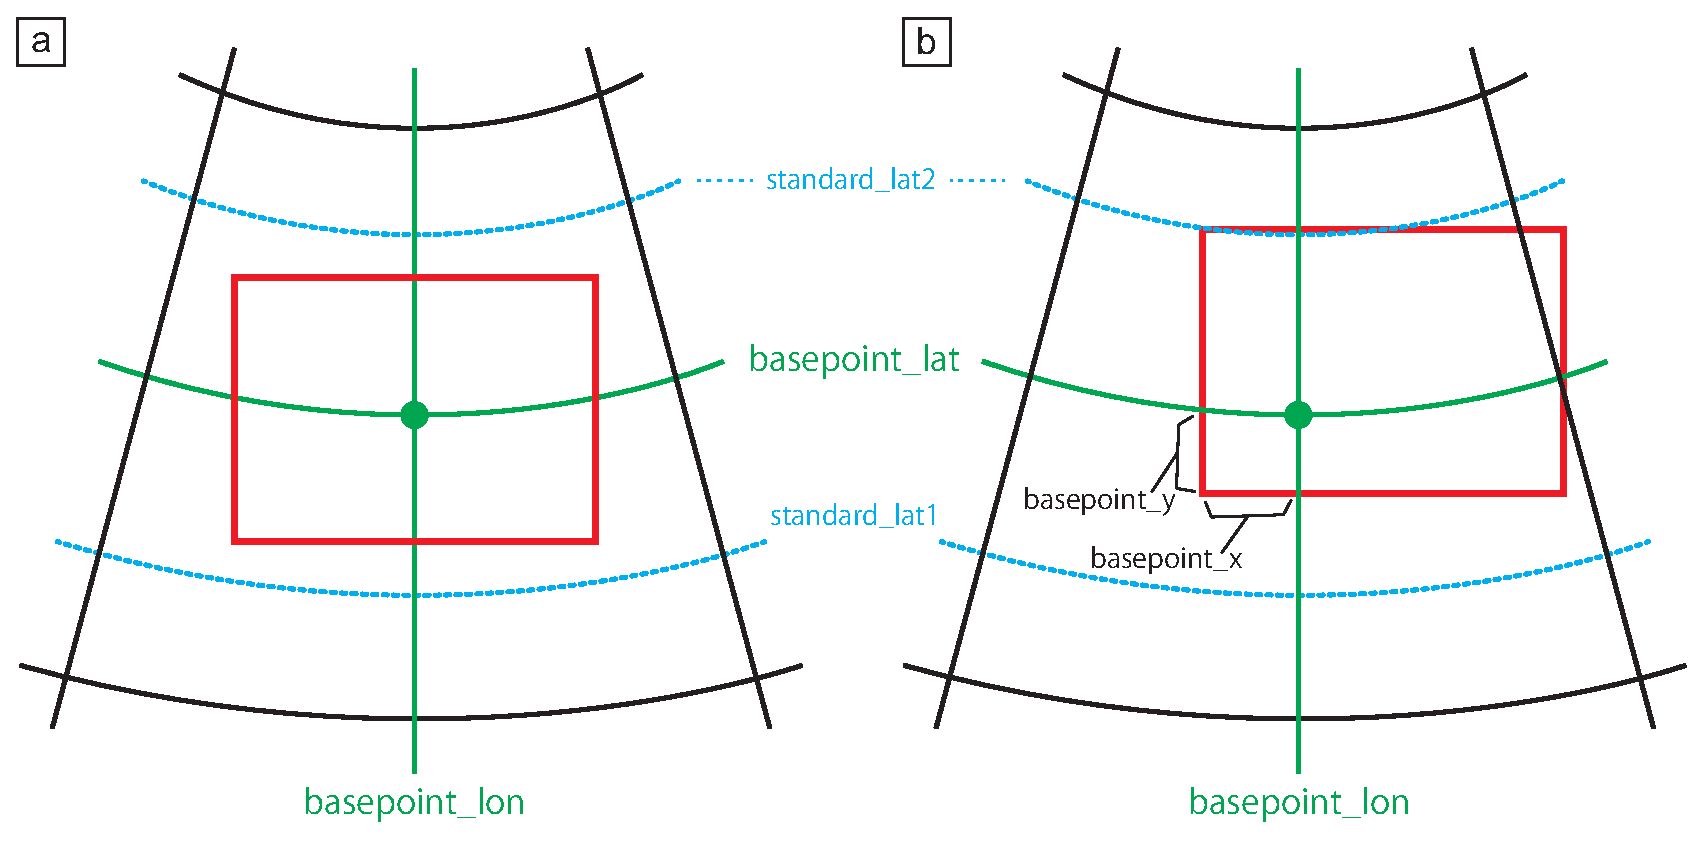
\includegraphics[width=0.8\hsize]{./figure/LC_latlon_xy.eps}\\
  \caption{投影中心と計算領域の関係:(a)はデフォルト設定の場合、(b)は投影中心の位置を計算領域中心からずらした場合。
  赤線の矩形が計算領域を表す。}
  \label{fig:map_lc}
\end{center}
\end{figure}
